% Documents setup
\documentclass[11pt]{book}\usepackage[]{graphicx}\usepackage[]{color}
%% maxwidth is the original width if it is less than linewidth
%% otherwise use linewidth (to make sure the graphics do not exceed the margin)
\makeatletter
\def\maxwidth{ %
  \ifdim\Gin@nat@width>\linewidth
    \linewidth
  \else
    \Gin@nat@width
  \fi
}
\makeatother

\definecolor{fgcolor}{rgb}{0.345, 0.345, 0.345}
\newcommand{\hlnum}[1]{\textcolor[rgb]{0.686,0.059,0.569}{#1}}%
\newcommand{\hlstr}[1]{\textcolor[rgb]{0.192,0.494,0.8}{#1}}%
\newcommand{\hlcom}[1]{\textcolor[rgb]{0.678,0.584,0.686}{\textit{#1}}}%
\newcommand{\hlopt}[1]{\textcolor[rgb]{0,0,0}{#1}}%
\newcommand{\hlstd}[1]{\textcolor[rgb]{0.345,0.345,0.345}{#1}}%
\newcommand{\hlkwa}[1]{\textcolor[rgb]{0.161,0.373,0.58}{\textbf{#1}}}%
\newcommand{\hlkwb}[1]{\textcolor[rgb]{0.69,0.353,0.396}{#1}}%
\newcommand{\hlkwc}[1]{\textcolor[rgb]{0.333,0.667,0.333}{#1}}%
\newcommand{\hlkwd}[1]{\textcolor[rgb]{0.737,0.353,0.396}{\textbf{#1}}}%
\let\hlipl\hlkwb

\usepackage{framed}
\makeatletter
\newenvironment{kframe}{%
 \def\at@end@of@kframe{}%
 \ifinner\ifhmode%
  \def\at@end@of@kframe{\end{minipage}}%
  \begin{minipage}{\columnwidth}%
 \fi\fi%
 \def\FrameCommand##1{\hskip\@totalleftmargin \hskip-\fboxsep
 \colorbox{shadecolor}{##1}\hskip-\fboxsep
     % There is no \\@totalrightmargin, so:
     \hskip-\linewidth \hskip-\@totalleftmargin \hskip\columnwidth}%
 \MakeFramed {\advance\hsize-\width
   \@totalleftmargin\z@ \linewidth\hsize
   \@setminipage}}%
 {\par\unskip\endMakeFramed%
 \at@end@of@kframe}
\makeatother

\definecolor{shadecolor}{rgb}{.97, .97, .97}
\definecolor{messagecolor}{rgb}{0, 0, 0}
\definecolor{warningcolor}{rgb}{1, 0, 1}
\definecolor{errorcolor}{rgb}{1, 0, 0}
\newenvironment{knitrout}{}{} % an empty environment to be redefined in TeX

\usepackage{alltt}

\usepackage{tabu} % https://tex.stackexchange.com/questions/50332/vertical-spacing-of-a-table-cell

% Location of the csas-style repository: adjust path as needed
\newcommand{\locRepo}{csas-style}

% Use the style file in the csas-style repository (res-doc.sty)
\usepackage{\locRepo/res-doc}

% Headers and footers
\lhead{Draft working paper --- Do not cite or circulate}
% \lhead{}
\rhead{}
% \rfoot{DRAFT - DO NOT CITE}

%%%% Commands for title page etc %%%%%

% Publication year
\newcommand{\rdYear}{YYYY}

% Publication month
\newcommand{\rdMonth}{Month}

% Report number
\newcommand{\rdNumber}{XXX}

% Title
\newcommand{\rdTitle}{A Data Synopsis Report for British Columbia Groundfish}

% Author names separated by commas and ', and' for the last author in the format 'M.H. Grinnell' (use \textsuperscript{n} for addresses)
\newcommand{\rdAuth}{Sean C. Anderson\textsuperscript{1}, Elise A.
Keppel\textsuperscript{1}, Other Possible Authors}

% Author names reversed separated by commas in the format 'Grinnell, M.H.'
\newcommand{\rdAuthRev}{Anderson, S.C., Keppel, E.A., Other Possible Authors.}

% Author addresses (use \textsuperscript{n})
\newcommand{\rdAuthAddy}{
\textsuperscript{1}Pacific Biological Station\\
Fisheries and Oceans Canada, 3190 Hammond Bay Road\\
Nanaimo, British Columbia, V9T 6N7, Canada
}

% Name of file with abstract and resume (see \abstract and \frenchabstract for requirements)
\newcommand{\rdAbstract}{
\abstract{}

[English abstract here.]

\frenchabstract{
[French title ici.]
}

[French abstract ici.]}

%%%% End of title page commands %%%%%

\pdfcompresslevel=5 % faster PNGs

\bibliographystyle{csas-style/res-doc}

\usepackage{amsmath}
\usepackage{bm}
% Let it begin
\IfFileExists{upquote.sty}{\usepackage{upquote}}{}
\begin{document}

% More custom variables

% Variables
% \newcommand{\fishName}{Pacific Herring}
% \newcommand{\scienceName}{\emph{Clupea pallasii}}

% Make the first few pages
\frontmatter



\section{INTRODUCTION} \label{sec:introduction}


The combination of fishery dependent data, such as catch and effort, and fishery
independent survey data, such as biomass indices and age compositions, form the
backbone of most fisheries stock assessment. Fisheries and Oceans Canada (DFO)
at the Pacific Biological Station (PBS) manages vast quantities of such data on
groundfish species in British Columbia (BC). However, we (DFO Science Branch, Pacific
Region stock assessment scientists) lack the capacity to conduct formal stock
assessments for most stocks annually, and therefore, much of these data are not
regularly published or readily accessible.

As one step to address this problem, we have created a data synopsis report to
give a snapshot of long-term and recent population and fishing trends and data
availability for all major British Columbia groundfish stocks of commercial and
conservation interest. The report is an extension of the data scorecard concept
discussed at a Canadian Science Advisory Secretariat (CSAS) Regional Peer Review
Meeting in May 2016 \citep{macdougall2016}. We plan to publish this report as
a CSAS Research Document in its first year and to update the report annually as
a CSAS Science Response in subsequent years. The report generation is fully
automated --- pulling data from databases, fitting models, generating
visualizations, and stitching the document together to facilitate rapid
publication.

Our (the authors') goals with this report are to (1) facilitate groundfish
scientists and managers regularly reviewing trends in survey indices and stock
composition across all stocks to potentially flag stocks for prioritized
assessment; (2) generate standardized datasets, biological model fits, and
visualizations that will help assessment scientists develop operating models and
select candidate management procedures as part of a planned management procedure
framework for data-limited and data-moderate groundfish stocks; and (3) increase
data transparency between Fisheries and Oceans Canada, the fishing industry,
First Nations, non-governmental organizations, and the general public.

\subsection{REPORT STRUCTURE}

The synopsis report is comprised of two-page species-by-species subsections that
visually synthesize most available data for each species. The report focuses on
the most important species to track for commercial and conservation concern, as
outlined in the current BC groundfish strategic plan, and focuses on the surveys
and data types applicable to the widest array of these fish stocks. Currently,
we have focused on the 31 A-level species, which are identified as the main species
of commercial and conservation interest. The strategic plan also includes a set
of B-level species (number TODO), which may be added in a future update of the report.

% TODO: hake
% TODO: add cosewic

Each set of pages for a single species is laid out in the same way. A set of
pages starts with the species common name, the species scientific name, and the
DFO species code, which usually corresponds to the page number referencing the
species in \citet{hart1988}. The figures themselves are laid out such
that the first page has survey timeseries trends and spatial patterns on the
left and commercial timeseries and spatial patterns on the right. The second
page is focused on biological samples. This page begins at the top with length and age
data and their relationship with each other, then shows data on maturity, and
finishes with an overview of available numbers of sampled fish across all survey
and commercial samples for various biological measurements.

In terms of surveys, we have focused on the Synoptic Bottom Trawl surveys, the
Outside Hard Bottom Long Line surveys (HBLL; alternatively referred to as the
Pacific Halibut Management Association, PHMA, surveys), and the International
Pacific Halibut Commission (IPHC) surveys (Fig.~\ref{fig:ss-maps}) because these provide the greatest
spatial and taxonomic coverage of the stocks in this report. As an example, we
are not showing biomass index trends or maps from the Sablefish trap surveys,
since these are highly selective for Sablefish. However, we do include counts of
available fish specimens from biological samples on all surveys and fit
biological models such as growth models to all available data.

\begin{knitrout}
\definecolor{shadecolor}{rgb}{0.969, 0.969, 0.969}\color{fgcolor}\begin{kframe}


{\ttfamily\noindent\itshape\color{messagecolor}{\#> Loading required package: Rcpp}}\end{kframe}\begin{figure}[htbp]

{\centering \includegraphics[width=\textwidth]{knitr-figs/ss-maps-1} 

}

\caption[Synoptic bottom trawl survey boundaries (left) and Outside Hard Bottom Long Line survey boundaries (right)]{Synoptic bottom trawl survey boundaries (left) and Outside Hard Bottom Long Line survey boundaries (right). The colours matches the colour coding through the rest of the report.}\label{fig:ss-maps}
\end{figure}


\end{knitrout}

Following the species-by-species visualizations, we include a section providing
details on the data extraction from the relational databases that hold the raw
data, a section providing details on the models that underlie some of the
visualizations, and finally a bibliography including all references listed
on the figure pages themselves. In navigating the report, we suggest that the
report is best viewed in a PDF two-page view so that all the plots for a single
species can be viewed at once. We also note that the table of contents and
references are clickable hyperlinks to facilitate navigation.

We made a number of overarching design decisions in structuring the report:

\begin{resdoclist}

\item Each species is displayed with the same layout to facilitate finding
  a type of data, comparing stocks, and identifying missing data via empty
  plots.

\item We have limited the report to two pages per species so that all plots can
  be laid out at once on a screen in a PDF. The data presentation is dense, but
  we believe there is value in being able to compare all the data for a species
  at once.

\item The colours representing the various surveys are held constant to
  facilitate tracing a single survey throughout the plots.

\item The colour scales are consistent for the survey maps and survey biological
  specimen number plots and for the commercial catch per unit effort maps and
  commercial biological specimen number plots (the bottom plots on both pages).

\item Data on female fish are always shown in front of data on male fish and
  are either coloured or black whereas males are always indicated with light
  grey. We did this to focus mainly on female fish, which are often more
  important in stock assessment models.

\end{resdoclist}

\subsection{CAVEATS}

There are many caveats when interpreting this report. First, the synopsis report
is not intended to be a substitute for stock assessment. For example, although
relative biomass indices from surveys can indicate the biomass trend for
a species in an area, such information is best combined with other information
such as removals by commercial catches and information on the age- or
length-composition of the stock to make conclusions about about the status of
a stock.
Second, biomass indices from trawl or longline surveys and commercial catch per
unit effort indices need careful interpretation on a stock-by-stock basis. We
have attempted to flag survey index trends that may be especially suspect either
because of high survey variability or because of a small fraction of trawl or
long line sets containing the species, but this is not a guarantee in itself.
Survey indices are not always representative of abundance for a variety of
reasons --- changes through time, including fish behavioural changes, could also
result in biases through time. Commercial catch per unit effort (CPUE)
timeseries, even when standardized for consistent time of year, depth, latitude,
and vessel need to be considered even more carefully. There are a multitude of
reasons why commercial CPUE trends may not represent underlying trends in
abundance \citep[e.g.][]{harley2001}. Nonetheless, we think there is value in
transparently displaying the available data for all species.

To be continued \ldots

\subsection{UPDATE SCHEDULE}

We plan to publish annual updates of this synopsis report as Science Response
documents. These annual updates will include another year of data and any
important corrections to the data, text, or visualizations. On a less frequent
basis we will consider making any larger changes to the structure or content of
the groundfish data synopsis report. We will consider these larger possible
revisions approximately every three years.

\subsection{GFPLOT AND GFSYNOPSIS R PACKAGES}

As stated above, one goal of this report is to generate standardized data sets,
model fits, and visualizations to facilitate stock assessment. We intend for the
data extraction and plots developed here to be useful for the upcoming
management-procedure framework for data-limited and data-moderate groundfish
stocks in BC, but also for the preparation of other groundfish stock assessments
and to facilitate data-to-document workflows that go straight from databases to
the final report via code and can be quickly updated in future years. To that
end, all data extraction, data manipulation, model fitting, and visualization
for this report is accomplished via the R package gfplot, which the authors
developed for this purpose. The specific layout and tools needed to make this
report are created with a second R package, gfsynopsis. Both packages (but not
the data itself) are publicly available on GitHub:\\
\url{https://github.com/pbs-assess/gfplot}\\
\url{https://github.com/pbs-assess/gfsynopsis}.

\subsection{ACKNOWLEDGEMENTS}

We are grateful for the ongoing collaboration between DFO, commercial fishers,
First Nations, and non-governmental organizations, which has made the collection
of the valuable data that underlies this report possible. We thank the project's
steering committee (Greg Workman, Robyn Forrest, Dana Haggarty, Andrew Edwards,
Chris Grandin, and Rob Kronlund) for invaluable input into the report design and
feedback throughout its production. We thank Christie Whelan for her support
initiating this project. We thank Norm Olsen, Maria Surry, and Malcolm Wyeth for
providing support on data extraction and general database structure and content.
We thank the participants of the peer review meeting on tiered approaches in May
2016, which included a data scorecard by Norm Olsen, from which this report
takes inspiration. We also thank Norm Olsen for his work on GFASTeR, which parts
of the code for this project are based on.


\clearpage

\section{PLOT DESCRIPTIONS} \label{sec:doc-background}

%<<data, child='doc/plot-descriptions.Rnw'>>=
%@

\clearpage

\section{SYNOPSIS PLOTS} \label{sec:plot-pages}

This section contains the main species-by-species data visualizations. Each
species is shown on two pages with the same layout used throughout. See
Section~\ref{sec:doc-background} for figure captions. The species are ordered
according to DFO species codes.
The table of contents at the beginning of the document includes links to the
various species pages.

%<<plots, child='doc/02-plots.Rnw'>>=
%@

\clearpage

\section{DATA EXTRACTION DETAILS} \label{sec:data}


Commercial and research catch, effort, and biological data for groundfish are
archived by the Groundfish Data Unit (Fisheries and Oceans Canada, Science
Branch, Pacific Region) and housed in a number of relational databases.
Historical commercial catch and effort data from 1954--2006/2007 are housed in
GFCatch, PacHarvTrawl, PacHarvHL, and PacHarvSable, depending on the fishery and
time period. Modern (2006/2007 to present) commercial catch data are housed in
GFFOS, a groundfish-specific view of the Fishery Operations System (FOS)
database (Fisheries and Oceans Canada, Fisheries and Aquaculture Management,
Pacific Region). Research survey data and commercial biological data from the
1940s to present are housed in GFBio, the Groundfish Biological Samples
database.

We developed a package gfplot for the statistical software R to automate data
extraction from these databases in a consistent, reproducible manner. The
functions extract data using SQL queries, developed with support from the
Groundfish Data Unit, which select and filter for specific data depending on the
analyses for which they will be used. The SQL file names mentioned in this
section can be viewed at
\url{https://github.com/pbs-assess/gfplot/tree/master/inst/sql} and may be
archived in the final version of this document.

We extracted commercial catch with \texttt{get-catch.sql}. All landings and
discards are extracted by species, fishery sector, gear type and year, and are
not filtered in any further way.

We extracted commercial trawl catch per unit effort (CPUE) index data using
\texttt{get-cpue-index.sql} and we filter the data to include only records with
valid start and end dates (Table~\ref{tab:sql-cpue-index}). Catch (kg) and
effort (expressed in hours), year, gear type and Pacific Fishery Management Area
(PFMA) are extracted for each tow. Gear type, PFMA and minimum year are given as
arguments and are set at defaults of bottom trawl, all areas, and 1996,
respectively.

We extracted commercial trawl spatial CPUE data using
\texttt{get-cpue-spatial.sql}, pulling out latitude, longitude, gear type, catch
(kg) and tow time (hours) for every tow by species. The data are filtered to
extract only records with valid start and end dates, to remove records with
erroneous latitude and longitude values, and to include only records from the
groundfish trawl sector with positive tows since 2012 when the trawl footprint
was implemented (Table~\ref{tab:sql-cpue-spatial}).

We extracted commercial hook and line spatial CPUE data using
\texttt{get-cpue-spatial-ll.sql}, which pulls out latitude and longitude, gear
type, catch (pieces) and years for all fishing events (sets, as a unit of
effort) by species. The data are filtered to extract only records with valid
start and end dates, to remove records with erroneous latitude and longitude
values, and to only include records with hook and line gear with non-zero catch.
Data include all records since 2008 after implementation of the Integrated
Groundfish Management Plan (Table~\ref{tab:sql-cpue-spatial-ll}). CPUE is
represented by landed catch in pieces per fishing event (set). Discards are not
included in hook and line spatial CPUE because discarded pieces are not reliably
recorded in all years. Species names are given as an argument to the function.

We extracted survey biomass index data \texttt{get-survey-index.sql}. Calculated
bootstrapped biomass, year and survey series identification code (SSID) are
filtered for active records of the calculated biomass in the database
(Table~\ref{tab:sql-survey-index}). Species and SSID codes are given as
arguments to the function.

We extracted biological data using \texttt{get-survey-samples.sql} and
\texttt{get-comm-samples.sql} for research survey and commercial samples,
respectively. Records of all biological samples are extracted by species,
including available length, weight, age and maturity data. Records include
available metadata including PFMA, fishery, gear type, SSID and survey
identification code (SID, only available for research survey data), survey
sampling types, and sampling protocol codes for maturity and ageing data. Data
are filtered by the \texttt{TRIP\_SUBTYPE\_CODE} to extract either survey
(Table~\ref{tab:sql-surv-samp}) or commercial (Table~\ref{tab:sql-comm-samp})
samples. In addition, samples are designated as one of three sample descriptions
based on combinations of two codes relating to sampling protocols:
\texttt{SPECIES\_CATEGORY\_CODE} (Table~\ref{tab:spp-cat}) and
\texttt{SAMPLE\_SOURCE\_CODE} (Table~\ref{tab:samp-source}). Samples can be
designated as `unsorted samples' in which data were collected for all specimens
in the sample, or `sorted samples' where specimens were sorted or selected into
`keepers', which were sampled, and `discards' which were not sampled:

\begin{resdoclist}

\item Specimens with a species category code of 0 are of unknown species
  category and are not useable. Those with a species category code of 1
  (unsorted) and a sample source code of 0 (unknown) or 1 (unsorted), or with a
  species category code of 5 (remains) or 6 (fish heads only) and a sample
  source code of 1 (unsorted) are classified as `unsorted'.

\item Specimens with a sample source code of 2 (keepers) and a species category
  code of 1 (unsorted), 2 (sorted) or 3 (keepers), or with a species category
  code of 3 (keepers) and a sample source code of 1 (unsorted) are classified as
  `keepers'.

\item Specimens with a species category code of 4 (discards) and a sample source
  code of 1 (unsorted) or 3 (discards), or a sample source code of 3 (discards)
  and a species category code of 1 (unsorted) are `discards'.

\end{resdoclist}

In the synopsis report, we are only including unsorted biological samples. Data
are also filtered by \texttt{SAMPLE\_TYPE\_CODE} to extract only total or random
samples and exclude samples selected by specified criteria.

Age data extracted with the biological sample queries are filtered by
\texttt{AGEING\_METHOD\_CODE} to select current ageing methods verified with the
ageing lab at the Pacific Biological Station in order to remove experimental
ageing methods that may also be recorded in the database.

Maturity codes are assigned at the time of sampling following one of
conventions. The various conventions have different scales and classifications.
We worked with the survey staff, data team and biologists for the various taxa
to select which codes at and above which an individual fish is considered
'mature' in order to assign a maturity status to each specimen based on a
combination of maturity convention, maturity code and sex.

The ageing precision data are extracted with \texttt{get-age-precision.sql}.
Data are filtered to bring in only records for which a secondary (precision)
reading was performed by a different technician in addition to the primary
reading (Table~\ref{tab:sql-age-precision}).

\clearpage

\begin{table}[htpb]
\centering
\caption{Description of filters in SQL queries extracting commercial sample data from GFBio with \texttt{get-comm-samples.sql}.}
\label{tab:sql-comm-samp}
{\tabulinesep=1.6mm
\begin{tabu}{>{\raggedright\arraybackslash}m{2.8in}>{\raggedright\arraybackslash}m{3.2in}}
\toprule
Filters                                                                                       & Rationale                                                                                                                                 \\
\midrule
Filtered out \texttt{TRIP\_SUBTYPE\_CODE} \texttt{2, 3} (research trips)                      & To extract only commercial data                                                                                                           \\
Filtered for \texttt{SAMPLE\_TYPE\_CODE} \texttt{1, 2, 6, 7, 8} (random or total)             & To extract only those records of sample type 'random' or 'total'                                                                          \\
Filtered for \texttt{SPECIES\_CATEGORY\_CODE} \texttt{NULL, 0, 1, 3, 4, 5, 6, 7}              & To remove samples sorted on unknown criteria                                                                                              \\
Filtered for \texttt{SAMPLE\_SOURCE\_CODE} \texttt{NULL, 1, 2, 3}                             & To extract both sorted and unsorted samples for later filtration for desired analysis (removes stomach contents samples)                  \\
\bottomrule
\end{tabu}}
\end{table}


\begin{table}[htpb]
\centering
\caption{Description of filters in SQL queries extracting research survey sample data from GFBio with \texttt{get-survey-samples.sql}.}
\label{tab:sql-surv-samp}
{\tabulinesep=1.6mm
\begin{tabu}{>{\raggedright\arraybackslash}m{2.8in}>{\raggedright\arraybackslash}m{3.2in}}
\toprule
Filters                                                                              & Rationale                                                                                                                                          \\
\midrule
Filtered for \texttt{TRIP\_SUBTYPE\_CODE} \texttt{2, 3} (research trips)                      & To extract only research data                                                                                                             \\
Filtered for \texttt{SAMPLE\_TYPE\_CODE} \texttt{1, 2, 6, 7, 8} (random or total)             & To extract only those records of sample type 'random' or 'total'                                                                          \\
Filtered for \texttt{SPECIES\_CATEGORY\_CODE} \texttt{NULL, 0, 1, 3, 4, 5, 6, 7}              & To remove samples sorted on unknown criteria                                                                                              \\
Filtered for \texttt{SAMPLE\_SOURCE\_CODE} \texttt{NULL, 1, 2, 3}                             & To extract both sorted and unsorted samples for later filtration for desired analysis (removes stomach contents samples)                  \\
\bottomrule
\end{tabu}}
\end{table}

\begin{table}[htpb]
\centering
\caption{Description of filters in SQL queries extracting commercial trawl catch and effort data from \texttt{GFFOS.GF\_MERGED\_CATCH} with \texttt{get-cpue-index.sql}}
\label{tab:sql-cpue-index}
{\tabulinesep=1.6mm
\begin{tabu}{>{\raggedright\arraybackslash}m{2.8in}>{\raggedright\arraybackslash}m{3.2in}}
\toprule
Filters                                                                                                                            & Rationale                                                                 \\
\midrule
Filtered for \texttt{END\_DATE} \texttt{IS NOT NULL} AND {START\_DATE} \texttt{IS NOT NULL}                                        & To remove records with missing date                                       \\
Filtered for \texttt{YEAR(FE\_START\_DATE)} = \texttt{YEAR(FE\_END\_DATE)} and \texttt{FE\_END\_DATE} > \texttt{FE\_START\_DATE}   & To remove records with erroneous dates                                    \\
\bottomrule
\end{tabu}}
\end{table}

\begin{table}[htpb]
\centering
\caption{Description of filters in SQL queries extracting commercial trawl spatial catch per unit effort (kg/hr) from \texttt{GFFOS.GF\_D\_OFFICIAL\_CATCH} with \texttt{get-cpue-spatial.sql}}
\label{tab:sql-cpue-spatial}
{\tabulinesep=1.6mm
\begin{tabu}{>{\raggedright\arraybackslash}m{2.8in}>{\raggedright\arraybackslash}m{3.2in}}
\toprule
Filters                                                                                                            & Rationale                                                                 \\
\midrule
Filtered for \texttt{LAT} between 47.8 and 55 and \texttt{LON} between -135 and -122                               & To remove erroneous location records                                      \\
Filtered for \texttt{YEAR(BEST\_DATE)} greater than 2012                                                           & To extract only records since the trawl fishery footprint was established \\
Filtered for \texttt{YEAR(START\_DATE)} = \texttt{YEAR(END\_DATE)} and \texttt{END\_DATE} > \texttt{START\_DATE}   & To remove records with erroneous dates                                    \\
Filtered for \texttt{FISHERY\_SECTOR} = \texttt{GROUNDFISH TRAWL}                                                   & To extract only records in the groundfish trawl fishery                   \\
Filtered for \texttt{ISNULL(LANDED\_ROUND\_KG,0) + ISNULL(TOTAL\_RELEASED\_ROUND\_KG,0)} > 0                            & To extract only records with positive catch                               \\
\bottomrule
\end{tabu}}
\end{table}

\begin{table}[htpb]
\centering
\caption{Description of filters in SQL queries extracting commercial hook and line spatial catch per unit effort (kg/set) from \texttt{GFFOS.GF\_D\_OFFICIAL\_CATCH} with \texttt{get-cpue-spatial-ll.sql}}
\label{tab:sql-cpue-spatial-ll}
{\tabulinesep=1.6mm
\begin{tabu}{>{\raggedright\arraybackslash}m{2.8in}>{\raggedright\arraybackslash}m{3.2in}}
\toprule
Filters                                                                                                            & Rationale                                                                 \\
\midrule
Filtered for \texttt{LAT} between 47.8 and 55 and \texttt{LON} between -135 and -122                               & To remove erroneous location records                                      \\
Filtered for \texttt{YEAR(BEST\_DATE)} greater than or equal to 2008                                               & To extract only records since 2008 after implementation of IFMP           \\
Filtered for \texttt{YEAR(START\_DATE)} = \texttt{YEAR(END\_DATE)} and \texttt{END\_DATE} > \texttt{START\_DATE}   & To remove records with erroneous dates                                    \\
Filtered for \texttt{GEAR} IN \texttt{(HOOK AND LINE, LONGLINE, LONGLINE OR HOOK AND LINE)}                        & To extract only records in the hook and line fishery                      \\
\bottomrule
\end{tabu}}
\end{table}

\begin{table}[htp]
\centering
\caption{Description of filters in SQL queries extracting bootstrapped survey biomass index from \texttt{GFBio} with \texttt{get-survey-index}}
\label{tab:sql-survey-index}
{\tabulinesep=1.6mm
\begin{tabu}{>{\raggedright\arraybackslash}m{2.8in}>{\raggedright\arraybackslash}m{3.2in}}
\toprule
Filters                                                                                                            & Rationale                                                                \\
\midrule
Filter for \texttt{ACTIVE\_IND} 1                                                                                  & To extract only active (useable) bootstrapped index records              \\
\bottomrule
\end{tabu}}
\end{table}

\begin{table}[htp]
\centering
\caption{Description of filters in SQL queries extracting all age records with a precision test reading to determine aging precision from {GFBio} with \texttt{get\_age\_precision.sql}}
\label{tab:sql-age-precision}
{\tabulinesep=1.6mm
\begin{tabu}{>{\raggedright\arraybackslash}m{2.8in}>{\raggedright\arraybackslash}m{3.2in}}
\toprule
Filters                                                                                                            & Rationale                                                                \\
\midrule
Filter for \texttt{AGE\_READING\_TYPE\_CODE} 2, 3                                                                     & To extract primary and precision test readings                           \\
\bottomrule
\end{tabu}}
\end{table}

%
% \begin{table}[htp]
% \centering
% \caption{Description of SQL queries used for data extraction in which no filters were applied and all data were extracted}
% \label{tab:sql-no filters}
% {\tabulinesep=1.6mm
% \begin{tabu}{>{\raggedright\arraybackslash}m{2.8in}>{\raggedright\arraybackslash}m{3.2in}}
% \toprule
% SQL Query                                                                                           & Rationale                                                                                                                \\
% \midrule
% Extract commercial landings from \texttt{GFFOS.GF\_MERGED\_CATCH} with \texttt{get-catch.sql}       & To extract all landings and discards by fishery sector and gear                                                          \\
% Assign maturity status from \texttt{GFFOS.GFBio} with \texttt{maturity\_assignment.sql}             & Designates maturity code at and above which a sample assessed following a given maturity convention is considered mature \\
% \bottomrule
% \end{tabu}}
% \end{table}

\begin{knitrout}
\definecolor{shadecolor}{rgb}{0.969, 0.969, 0.969}\color{fgcolor}\begin{kframe}


{\ttfamily\noindent\color{warningcolor}{\#> Warning in gzfile(file, "{}rb"{}): cannot open compressed file '../../data-cache2/pbs-survey-sets.rds', probable reason 'No such file or directory'}}

{\ttfamily\noindent\bfseries\color{errorcolor}{\#> Error in gzfile(file, "{}rb"{}): cannot open the connection}}

{\ttfamily\noindent\bfseries\color{errorcolor}{\#> Error in eval(lhs, parent, parent): object 'd\_survey\_sets' not found}}

{\ttfamily\noindent\bfseries\color{errorcolor}{\#> Error in tbl\_vars(y): object 'meta' not found}}

{\ttfamily\noindent\bfseries\color{errorcolor}{\#> Error in `\$<-.data.frame`(`*tmp*`, species\_science\_name, value = character(0)): replacement has 0 rows, data has 31}}

{\ttfamily\noindent\bfseries\color{errorcolor}{\#> Error in `\$<-.data.frame`(`*tmp*`, species\_science\_name, value = character(0)): replacement has 0 rows, data has 31}}

{\ttfamily\noindent\bfseries\color{errorcolor}{\#> Error in .f(.x[[i]], ...): object 'species\_science\_name' not found}}

{\ttfamily\noindent\bfseries\color{errorcolor}{\#> Error in arrange\_impl(.data, dots): Evaluation error: object 'species\_code' not found.}}

{\ttfamily\noindent\bfseries\color{errorcolor}{\#> Error in `substr<-`(`*tmp*`, 1, 1, value = toupper(substr(x, 1, 1))): replacing substrings in a non-character object}}

{\ttfamily\noindent\bfseries\color{errorcolor}{\#> Error in names(age\_methods) <- c("{}Common name"{}, "{}Scientific name"{}, "{}Species code"{}, : 'names' attribute [4] must be the same length as the vector [3]}}\end{kframe}
\end{knitrout}

% latex table generated in R 3.5.0 by xtable 1.8-2 package
% Fri Jul 27 14:13:24 2018
\begin{table}[ht]
\centering
\caption{Ageing method codes from GFBio considered valid throughout the synopsis document for groundfish species in British Columbia. The ageing method codes were chosen with the help of the PBS Schlerochronology Lab. 1 $=$ `Otolith Surface Only', 3 $=$ ` Otolith Broken and Burnt', 17 $=$ `Otolith Broken and Baked (Break and Bake)', 6 $=$ `Dorsal Fin XS', 11 $=$ `Dorsal Spine', 12 $=$ `Vertebrae'.} 
\begin{tabular}{lll}
  \toprule
species_common_name & type & ageing_method_codes \\ 
  \midrule
Lingcod & A & 6 \\ 
  Pacific Cod & A & 6 \\ 
  Walleye Pollock & A & 7 \\ 
  Pacific Hake & A & 1, 3, 17 \\ 
  Rougheye/blackspotted  & A & 1, 3, 17 \\ 
  Pacific Ocean Perch & A & 1, 3, 17 \\ 
  Redbanded Rockfish & A & 1, 3, 17 \\ 
  Silvergray Rockfish & A & 1, 3, 17 \\ 
  Copper Rockfish & A & 1, 3, 17 \\ 
  Darkblotched Rockfish & A & 1, 3, 17 \\ 
  Widow Rockfish & A & 1, 3, 17 \\ 
  Yellowtail Rockfish & A & 1, 3, 17 \\ 
  Quillback Rockfish & A & 1, 3, 17 \\ 
  Bocaccio & A & 1, 3, 17 \\ 
  Canary Rockfish & A & 1, 3, 17 \\ 
  Redstripe Rockfish & A & 1, 3, 17 \\ 
  Yellowmouth Rockfish & A & 1, 3, 17 \\ 
  Yelloweye Rockfish & A & 1, 3, 17 \\ 
  Sablefish & A & 1, 3, 17 \\ 
  Arrowtooth Flounder & A & 1, 3, 17 \\ 
  Petrale Sole & A & 1, 3, 17 \\ 
  Rex Sole & A & 1, 3, 17 \\ 
  Southern Rock Sole & A & 1, 3, 17 \\ 
  Dover Sole & A & 1, 3, 17 \\ 
  English Sole & A & 1, 3, 17 \\ 
  Shortraker Rockfish & A & 1, 3, 4, 17 \\ 
  Shortspine Thornyhead & A & 1, 3, 4, 17 \\ 
  Longspine Thornyhead & A & 1, 3, 4, 17 \\ 
  North Pacific Spiny Dogfish & A & 11 \\ 
  Big Skate & A & 12 \\ 
  Longnose Skate & A & 12 \\ 
   \bottomrule
\end{tabular}
\end{table}



% latex table generated in R 3.5.0 by xtable 1.8-2 package
% Fri Jul 27 14:13:24 2018
\begin{table}[ht]
\centering
\caption{Maturity convention codes (`Mat. conv. code'), maturity convention descriptions, sex, and the maturity convention value at which a fish is deemed to be mature for the purposes of the synopsis report. Note that fish may be considered mature at other maturity convention values in particular stock assessments where other values are chosen for specific reasons.} 
\begin{tabular}{rllr}
  \toprule
Mat. conv. code & Maturity convention description & Sex & Mature at \\ 
  \midrule
  1 & ROCKFISH (1977+) & M &   3 \\ 
    1 & ROCKFISH (1977+) & F &   3 \\ 
    4 & FLATFISH (1978+) & M &   3 \\ 
    4 & FLATFISH (1978+) & F &   3 \\ 
    6 & PACIFIC COD (1973-75) & M &   2 \\ 
    6 & PACIFIC COD (1973-75) & F &   2 \\ 
    7 & PACIFIC COD (1975+) & M &   3 \\ 
    7 & PACIFIC COD (1975+) & F &   3 \\ 
    8 & LINGCOD (1985+) & M &   3 \\ 
    8 & LINGCOD (1985+) & F &   3 \\ 
   10 & DOGFISH & M &  90 \\ 
   10 & DOGFISH & F &  77 \\ 
   11 & PORT SAMPLES & M &   3 \\ 
   11 & PORT SAMPLES & F &   3 \\ 
   12 & THORNYHEAD SIMPLIFIED & M &   2 \\ 
   12 & THORNYHEAD SIMPLIFIED & F &   2 \\ 
   13 & AMR & M &   3 \\ 
   13 & AMR & F &   3 \\ 
   15 & ROCKFISH (1975-77) & M &   3 \\ 
   15 & ROCKFISH (1975-77) & F &   3 \\ 
   16 & SARDINES (I, M OR R) & M &   2 \\ 
   16 & SARDINES (I, M OR R) & F &   2 \\ 
   17 & SKATE (2002+) & M &   2 \\ 
   17 & SKATE (2002+) & F &   2 \\ 
   21 & GENERAL GROUNDFISH (LATE 1960'S-EARLY 1970'S) & M &   3 \\ 
   21 & GENERAL GROUNDFISH (LATE 1960'S-EARLY 1970'S) & F &   3 \\ 
   22 & SIMPLIFIED - OLD & M &   2 \\ 
   22 & SIMPLIFIED - OLD & F &   2 \\ 
   23 & MISC. SPECIES SIMPLIFIED & M &   2 \\ 
   23 & MISC. SPECIES SIMPLIFIED & F &   2 \\ 
   24 & LINGCOD 7-STAGE & M &   3 \\ 
   24 & LINGCOD 7-STAGE & F &   3 \\ 
   25 & HAKE-POLLOCK 7-STAGE & M &   3 \\ 
   25 & HAKE-POLLOCK 7-STAGE & F &   3 \\ 
   26 & RATFISH & M &   3 \\ 
   26 & RATFISH & F &   3 \\ 
   \bottomrule
\end{tabular}
\end{table}


% latex table generated in R 3.5.0 by xtable 1.8-2 package
% Fri Jul 27 14:13:24 2018
\begin{table}[ht]
\centering
\caption{Species category codes lookup table, which
  describes sampling protocols at the catch level.} 
\label{tab:spp-cat}
\begin{tabular}{rl}
  \toprule
Species Category Code & Species Category Description \\ 
  \midrule
  0 & Unknown \\ 
    1 & Unsorted \\ 
    2 & Sorted (unknown criterion) \\ 
    3 & Keepers \\ 
    4 & Discarded \\ 
    5 & Remains \\ 
    6 & Longline -- fish head only \\ 
    7 & Longline -- whole fish and fish head only \\ 
    8 & Longline/jig -- fish lost at rail/lost at surface \\ 
   \bottomrule
\end{tabular}
\end{table}


% latex table generated in R 3.5.0 by xtable 1.8-2 package
% Fri Jul 27 14:13:24 2018
\begin{table}[ht]
\centering
\caption{Sample source codes lookup table, which
  describes sampling protocols at the sample level.} 
\label{tab:samp-source}
\begin{tabular}{rl}
  \toprule
Sample Source Code & Sample Source Description \\ 
  \midrule
  0 & Unknown \\ 
    1 & Unsorted \\ 
    2 & Keepers \\ 
    3 & Discards \\ 
    4 & Stomach contents \\ 
   \bottomrule
\end{tabular}
\end{table}


\clearpage

\section{MODELLING DETAILS} \label{sec:modelling-details}


\subsection{SURVEY RELATIVE BIOMASS INDEX TRENDS} \label{sec:survey-trend-models}

Details on the design of the various surveys referenced in this report can be
found in the following documents:

\begin{resdoclist}

\item Synoptic Survey, Queen Charlotte Sound (SYN QCS):  \citep{wyeth2018synqcs}

\item Synoptic Survey, West Coast Vancouver Island (SYN WCVI):
  \citep{wyeth2017synwcvi}

\item Synoptic Survey, Hecate Strait (SYN HS): \citep{wyeth2018synhs}

\item Synoptic Survey, West Coast Haida Gwaii (SYN WCHG):
  \citep{wyeth2018synwchg}

\item Hard Bottom Longline Survey, Outside (HBLL OUT): \citep{dfo2018ifmp}

\item Hard Bottom Longline Survey, Inside (HBLL INS): \citep{lochead2004irf}

\item Hecate Strait Multispecies Assemblage Survey (MSA HS):
  \citep{fargo1984hsmsa,westrheim1984hsmsa}

\item International Pacific Halibut Commission fishery independent survey (IPHC
  FISS): \citep{flemming2012iphc}

\end{resdoclist}

We calculated the trawl and longline survey relative biomass index trends from
the same design-based bootstrap approach used in recent BC groundfish stock
assessment reports. The code to perform the calculations was originally written
by Norm Olsen at Pacific Biological Station and is automatically applied to the
available survey data to populate the GFBio database. We extracted the relative
biomass values directly from GFBio. Nonetheless, we have included the relevant
equations below for clarity.

\subsubsection{TRAWL SURVEYS}

For all trawl surveys, and for a given species, we calculated the relative
biomass density $B$ in year $y$ as:

\begin{equation}
  B_y = \sum_{i = 1}^k C_{y,i} A_i
\end{equation}

where $C_{y,i}$ represents the mean CPUE in kg/km\textsuperscript{2} for the
species in year $y$ and stratum $i$, $A_i$ represents the area of stratum $i$ in
km\textsuperscript{2}, and $k$ represents the number of strata. We calculated
the CPUE ($C_{y,i}$) for a given species in year $y$ and stratum $i$ as:

\begin{equation}
  C_{y,i} = \frac{\sum_{j = 1}^{n_{y,i}} \left( W_{y,j} / D_{y,j} w_{y,j}\right)}{n_{y,i}}
\end{equation}

where $W_{y,j}$ represents the catch weight (kg) for the species in year $y$,
stratum $i$, and tow $j$; $D_{y,j}$ represents the distance travelled in km by
tow $j$ in year $y$; $w_{y,j}$ represents the net opening width in km for year
$y$ and tow $j$; and $n_{y,i}$ represents the number of tows in year $y$ and
stratum $i$.

\subsubsection{LONG-LINE SURVEYS}

For all long-line surveys, and for a given species, we calculated the relative
biomass density $B$ in year $y$ as:

\begin{equation}
  B_y = \sum_{i = 1}^k C_{y,i} A_i
\end{equation}

where $C_{y,i}$ represents the mean CPUE in parts (fish) per
km\textsuperscript{2} for the species in year $y$ and stratum $i$, $A_i$
represents the area of stratum $i$ in km\textsuperscript{2}, and $k$ represents
the number of strata. We calculated the CPUE ($C_{y,i}$) for a given species in
year $y$ and stratum $i$ as:

\begin{equation}
  C_{y,i} = \frac{\sum_{j = 1}^{n_{y,i}} \left( N_{y,j} / H_{y,j} w_{y,j}\right)}{n_{y,i}}
\end{equation}

where $N_{y,j}$ represents the number of fish caught for the species in year
$y$, stratum $i$, and set $j$; $H_{y,j}$ represents the number of hooks $\times$
the hook spacing in km in set $j$ in year $y$; $w_{y,j}$ represents an arbitrary
swept width of 30 feet or 0.009144 km for year $y$ and tow $j$; and $n_{y,i}$
represents the number of sets in year $y$ and stratum $i$. The hook spacing is
18 feet or 0.0054864 km for the IPHC survey and 8 feet or 0.0024384 km for
the inside and outside HBLL surveys.

\subsubsection{BOOTSTRAPPED CONFIDENCE INTERVALS}

We calculated bootstrap confidence intervals on $B_y$ by repeatedly calculating
$B_y$ given the above equations but each time re-sampling, with replacement, from
the available tows within each strata. We drew 1000 bootstrap replicates of
$B_y$, $B_y^{\mathrm{rep}}$, and calculated 95\% quantile-based confidence
intervals on $B_y^{\mathrm{rep}}$.


\subsection{SPATIAL MODELLING OF SURVEY BIOMASS} \label{sec:spatial-modeling}


We modelled the expected biomass density in space for each species using
geostatistical models applied to data from the fisheries independent bottom
trawl and long line surveys (e.g.~Figure~\ref{fig:survey-maps}). Our modeling
approach is consistent with recent models used for spatiotemporal index
standardization of fish populations
\citep[e.g.][]{shelton2014,ward2015,thorson2015,thorson2016}. Such models have
been shown, for example, to improve estimates of rockfish abundance and
distribution \citep{shelton2014} and improve precision when estimating relative
abundance indices for groundfish \citep{thorson2015}. Our specific model follows
the implementation in \citet{shelton2018} closely and is implemented with INLA
\citep{rue2009, lindgren2015} via R \citep{rcoreteam2018}, which enables rapid
Bayesian model fitting for these large spatial data sets via the integrated
nested Laplace approximation of the posterior distribution.

At a high level, these models predict relative biomass in space as a continuous
process with a quadratic effect for bottom depth, a random effect spatial
surface that represents an amalgamation of spatial processes not explicitly
included in the model, and an observation error component. After fitting the
model to survey sets from trawl or longline surveys, the model is then projected
to a fine-scale 2$\times$2 km grid in a UTM 9 projection to derive estimates of
biomass throughout the survey domain.

Similarly to the catch per unit effort index standardization (explained in
Section \ref{sec:cpue-models}), we fit these models as `delta' models that
combine a model explaining the probability of occurrence of a species in a set
with a model explaining the expected biomass in a set given that the species has
been caught. The probability from the first model is multiplied by the expected
biomass from the second model to derive the overall estimate of relative
biomass.

We fit the binomial occurrence models (denoted with a superscript $B$), which
predict the probability of occurrence of a given species at location $s$,
$\pi_s^B$ as a logistic GLMM (Generalized Linear Mixed-effects Model):

\begin{align}
  y_\mathbf{s}^B &\sim \mathrm{Binomial}(\pi_\mathbf{s}^B)\\
  \mathrm{logit} \left(\pi_\mathbf{s}^B \right) &= \bm{X}_\mathbf{s}^B \bm{\beta}^B + \epsilon_\mathbf{s}^B,
\end{align}

where

\begin{equation}
  \mathrm{logit}\left(\pi \right) = \log \left( \frac{\pi}{1 - \pi} \right).
\end{equation}

The spatial random effects $\epsilon_\mathbf{s}^B$ are assumed to be drawn from
a multivariate normal distribution with covariance matrix
$\bm{\Phi}_\mathbf{s}^B$ that is centered on zero:

\begin{equation}
  \epsilon_\mathbf{s}^B \sim \mathrm{MVNormal} \left( \bm{0}, \bm{\Phi}_\mathbf{s}^B \right).
\end{equation}

We fit the positive model (denoted with a superscript $G$ for Gamma) as a Gamma
GLMM with a similar structure for the spatial random effects:

\begin{align}
  y_\mathbf{s}^G &\sim \mathrm{Gamma} \left( \bm{\mu}_\mathbf{s}^G, \phi^G \right)\\
  \log \left( \bm{\mu}_\mathbf{s}^G \right) &= \bm{X}_\mathbf{s}^G \bm{\beta}^G + \epsilon_\mathbf{s}^G\\
  \epsilon_\mathbf{s}^G &\sim \mathrm{MVNormal} \left( \bm{0}, \bm{\Phi}_\mathbf{s}^G \right)
\end{align}

We modeled the covariance for the spatial random effects in both the occurrence
and positive models as a function of distance with the Mat\'ern function. The
Mat\'ern function describes the covariance between spatial locations $s_j$ and
$s_k$ as:

\begin{equation}
  \Phi\left( s_j,s_k \right) = \tau^2/\Gamma(\nu)2^{\nu - 1}
    (\kappa d_{jk})^\nu K_\nu \left( \kappa d_{jk} \right),
\end{equation}

where $\tau^2$ represents the spatial variance, $\Gamma$ represents the Gamma
function, $K_\nu$ represents the Bessel function, $d_{jk}$ represents the
Euclidean distance between locations $s_j$ and $s_k$, and $\kappa$ represents a
scaling parameter that is estimated. The parameter $\nu$ controls the smoothness
of the covariance function. We set $\nu = 3/2$, as is commonly done when fitting
similar spatial models \citep[e.g.][]{ward2015, thorson2015, ono2016,
shelton2018}, which lets the covariance function be more flexible than an
exponential covariance function but still be differentiable
\citep{rasmussen2004}.

At this stage we drew 1000 samples from the posterior distributions of
$\pi_\mathbf{s}^B$ and $\mu_\mathbf{s}^G$ and combined them to estimate the unconditional posterior distribution of expected biomass in each point on a 2x2km spatial grid, $\mu_\mathbf{s}$ as:

\begin{equation}
  \mu_\mathbf{s} = \pi_\mathbf{s}^B \cdot \mu_\mathbf{s}^G.
\end{equation}

For the purposes of the maps, we summarized the posteriors by their median
values. See Figures~\ref{fig:example-survey-maps-syn} and
\ref{fig:example-survey-maps-hbll} for examples of these sub-component binary
and positive models and the combined model. We placed Normal(0, 5) priors on
coefficients relating standardized depth and standardized depth squared to the
responses and Normal(0, 20) priors on the intercepts. Note that our notation is
Normal(mean, standard deviation) not Normal(mean, variance) following the
convention used by the Bayesian software Stan \citep{rstan2018}.

We fit the four synoptic survey data sets separately, because only two of the
surveys are conducted each year and the surveys are disjointed in space and
time. We combined the predictions to generate the map plots, but labelled the
years the various surveys were conducted in. Currently, we are fitting the HBLL
surveys as one dataset, although we plan to separate the north and south surveys
since they are also conducted in offset years. We have projected the IPCC model
estimates back to the original station locations for simplicity and to avoid
having to derive a reasonable survey domain polygon.

% We will fit one model predicting the presence vs. absence of Pacific ocean perch
% in a given tow and another model predicting the biomass of Pacific ocean perch
% given that a tow includes the species. One is a binomial GLMM with a logit link.
% The other is a lognormal GLMM with a log link. Both are currently modelled with
% a squared exponential covariance function. Alternatives would include an
% exponential or Matern covariance function, but likely make little difference
% here.
%
% TODO: the following is very incomplete:
%
% The models can be described as:
%
% \begin{align}
%   g(\mu_{s}) &= \beta_0 + \beta_1 T_s + \beta_2 T^2_s + \gamma_{s}, \\
%   \gamma_{s} &\sim \mathrm{MVN}\left(0, \mathbf{\Sigma}_{s}\right),
% \end{align}
%
% where $g$ represents a link function (log or logit), $\mu_{s}$ represents the
% mean at spatial location $s$, $T$ represents bottom temperature, the $\beta$s
% represent estimated coefficients, $\gamma_{s}$ represents a Gaussian random
% field, and $\mathbf{\Sigma}_{s}$ represents a covariance matrix.
%
% The squared exponential covariance function models the correlation between
% points $i$ and $j$ as $H(\delta_{ij}) = \exp \left(- \delta_{ij}^2
% / 2 \theta_{\mathrm{GP}} \right)$, where $\delta_{ij}$ is the distance between
% points $i$ and $j$ and $\theta_{\mathrm{GP}}$ controls how steeply correlation
% declines with distance (GP = Gaussian process). For a given set of
% $\delta_{ij}$, large values of $\theta_{\mathrm{GP}}$ correspond to smooth
% spatial patterns and small values correspondence to wiggly spatial patterns.
%
% The elements of the covariance matrix $\mathbf{\Sigma}$ at the $m$ knot
% locations are then defined as $\mathbf{\Sigma}_{ij}^* = \sigma_{\mathrm{GP}}^2
% \exp \left( -\delta_{ij}^2 / 2 \theta_{\mathrm{GP}} \right)$ with the spatial
% variance parameter $\sigma_{\mathrm{GP}}^2$ scaling the amplitude of the spatial
% deviations and the $*$ denoting a symbol referring to the knot locations as
% opposed to the sample locations.

% TODO: add units to the color scale or the caption on this and subsequent
% figures

\begin{knitrout}
\definecolor{shadecolor}{rgb}{0.969, 0.969, 0.969}\color{fgcolor}\begin{kframe}


{\ttfamily\noindent\bfseries\color{errorcolor}{\#> Error in gzfile(file, "{}rb"{}): cannot open the connection}}

{\ttfamily\noindent\bfseries\color{errorcolor}{\#> Error in plot\_survey\_sets(pred\_dat, raw\_dat, fill\_column = fill\_column, : object 'eg\_syn' not found}}

{\ttfamily\noindent\bfseries\color{errorcolor}{\#> Error in plot\_survey\_sets(pred\_dat, raw\_dat, fill\_column = fill\_column, : object 'eg\_syn' not found}}

{\ttfamily\noindent\bfseries\color{errorcolor}{\#> Error in plot\_survey\_sets(pred\_dat, raw\_dat, fill\_column = fill\_column, : object 'eg\_syn' not found}}

{\ttfamily\noindent\bfseries\color{errorcolor}{\#> Error in arrangeGrob(...): object 'bin' not found}}\end{kframe}
\end{knitrout}

\begin{knitrout}
\definecolor{shadecolor}{rgb}{0.969, 0.969, 0.969}\color{fgcolor}\begin{kframe}


{\ttfamily\noindent\bfseries\color{errorcolor}{\#> Error in gzfile(file, "{}rb"{}): cannot open the connection}}

{\ttfamily\noindent\bfseries\color{errorcolor}{\#> Error in plot\_survey\_sets(pred\_dat, raw\_dat, fill\_column = fill\_column, : object 'eg\_hbll' not found}}

{\ttfamily\noindent\bfseries\color{errorcolor}{\#> Error in plot\_survey\_sets(pred\_dat, raw\_dat, fill\_column = fill\_column, : object 'eg\_hbll' not found}}

{\ttfamily\noindent\bfseries\color{errorcolor}{\#> Error in plot\_survey\_sets(pred\_dat, raw\_dat, fill\_column = fill\_column, : object 'eg\_hbll' not found}}

{\ttfamily\noindent\bfseries\color{errorcolor}{\#> Error in arrangeGrob(...): object 'bin' not found}}\end{kframe}
\end{knitrout}




\clearpage

\subsection{CPUE INDEX STANDARDIZATION} \label{sec:cpue-models}

We present two commercial bottom trawl catch per unit effort (CPUE) indices in
the synopsis report: a `raw' unstandardized timeseries and a `standardized' time
series (e.g.\ Figure~\ref{fig:trawl-cpue-index}). The standardized time series
follows the approach commonly employed for British Columbia groundfish stock
assessments of using a Generalized Linear Model (GLM) to account for the
confounding effects of month, depth, latitude, vessel, and DFO locality
(predesignated historical geographical locations) when calculating an annual
index value. We do this by fitting two GLMs: one to data representing whether or
not the species of interest (e.g. Pacific Cod for a Pacific Cod CPUE index) is
caught in a given tow (the `binary' model),
and a second model to data representing the CPUE conditional on a tow having caught
at least one of that species of interest (the `lognormal' model). This approach is
sometimes called a delta-lognormal GLM. These two model components can then be
combined to derive the final estimate of CPUE for a given year at a consistent
value for all the predictors, i.e. a consistent month, depth, latitude, vessel,
and DFO locality.

For depth and latitude, we binned the values into a sequence of bands to allow
for nonlinear relationships between these predictors and the response. For
latitude, we used bands that are 0.2 degrees wide, start at the 2\% quantile of
the latitude values for the specific region and end at the 98\% quantile of the
latitude values. We used this quantile method to algorithmically account for
outlying values that were often data recording errors and could cause problems
when fitting the models. We rounded the lowest latitude bin down to the nearest
0.2 latitude value and rounded to the upper latitude bin up to the nearest 0.2
  latitude value. For depth, we used the fishing capture depth binned into bands
  that are 50m wide. The bins start at the 1\% quantile of the depth values for
  the specific region and end at the 99\% quantile of the depth values. We
  rounded the lowest and highest bin values to 50m values similarly to the
  process for the latitude bins as described above.

Due to the multispecies nature of the BC groundfish fishery, it is necessary to
define rules about which vessels should be considered part of a `fleet'
with which to calculate a CPUE index. We follow the approach used in a number of
recent BC groundfish stock assessments by requiring vessels to have caught the
species in a certain number of tows across all years of interest, and to have
passed a certain threshold of positive trips (trips that recorded some of the
species) for a certain number of years. Our current implementation requires a
vessel to have recorded at least 100 positive tows since 1996 and to have
recorded at least four positive trips in at least four years since 1996. These
decisions are in line with recent BC groundfish stock assessments
\citep[e.g.][]{starr2017pollock}.

We fit the binomial model (denoted with a superscript $B$) as a logistic
regression:

\begin{align}
  y_i^B &\sim \mathrm{Binomial}(\pi_i^B)\\
  \mathrm{logit}\left(\pi_i^B\right) &= \bm{X}_i^B \bm{\beta}^B,
\end{align}

and $i$ represents a single tow, $y_i$ represents either a 1 if a tow caught the
species or a 0 if it did not, $\bm{X^B_i}$ represents a vector of predictors,
$\bm{\beta^B}$ represents a vector of coefficients, and $\pi_i^B$ represents the
estimated probability of observing the species in a tow. Details to follow on
the specific depth and latitude bands chosen.

We fit the lognormal model (denoted with a superscript $L$) as a linear model
fit to log-transformed response data:

\begin{equation}
  \log \left(y_i^L\right) \sim \mathrm{Normal} \left(\bm{X}_i^L \bm{\beta}^L, \sigma \right),
\end{equation}

where the symbols can be interpreted as before except that $y_i^L$ represents
the CPUE in kg per hour towed for a tow that did catch at least one of the
species, and $\sigma$ represents the standard deviation of unexplained residual
error.

We can then calculate the standardized estimate of CPUE for year $t$, $\mu_t$ as:

\begin{equation}
  \mu_t = \mathrm{logit}^{-1} \left(\bm{X}_r^B
    \bm{\beta}^B \right) \cdot \exp \left(\bm{X}_r^L \bm{\beta}^L \right)
\end{equation}

or

\begin{equation}
  \mu_t = \pi_t^B \cdot \exp \left(\bm{X}_r^L \bm{\beta}^L \right)
\end{equation}

where $\bm{X_r}$ represents a vector of predictors set to the reference ($r$)
levels with the year set to the year of interest. We chose the reference levels
as the most frequent level of each predictor in the positive-only data
\citep{maunder2004}. For example, we set the reference month as the most common
month observed in the dataset filtered for only tows where the species was
caught. This will have a minor effect on the shape of the final CPUE index
because of the multiplication of the binary and positive components.

Recent BC groundfish stock assessments have used a bootstrap approach to derive
estimates of uncertainty around standardized CPUE timeseries. This proved to be
computationally unfeasible to run for all the management areas and stocks in
this synopsis report. Therefore we wrote the model in the statistical software
TMB \citep{kristensen2016} and use standard errors ($\mathrm{SE}$) as calculated
by TMB on $\log (\mu_t)$ via the Delta method as is commonly done for such
models \citep[e.g.][]{thorson2015}. We then calculated the 95\% confidence
intervals as $\exp (\mu_t \pm 1.96 \mathrm{SE}_t)$.

We calculated the `raw' unstandardized timeseries is calculated using a similar
procedure but without any of the covariates other than a factor predictor for
each year. This is equivalent to calculating the geometric mean of CPUE each
year.

We tested our implementation of this index standardization model against
simulated data to ensure that (1) it can generate unbiased annual estimates and
(2) the confidence intervals have the correct coverage, i.e. the confidence
intervals contain the true known value at the expected frequency of 95\%. We
also compared our estimates qualitatively to recent estimates from similar
models in published assessments to ensure we derived similar timeseries.

For the simulation testing, as examples, we present results for two simulations
with 10 vessels, each vessel recording data from 15 tows, 20 years of data, and
lognormal observation error with standard deviation 0.35 (i.e., approximately
a CV of 0.35). The standardization model then accounts for vessel ID in both
a binary and positive component model. The delta model derives an unconditional
estimate of CPUE after combining the two component models. The parameter
estimates from the component models regularly fall along the one-to-one line of
unbiased and accurate prediction (e.g. Fig.~\ref{fig:cpue-sim-cross-val}) and
the unconditional estimates of CPUE and their confidence intervals regularly
include the true values with correct coverage (e.g.
Fig.~\ref{fig:cpue-sim-ts-val}).

\begin{knitrout}
\definecolor{shadecolor}{rgb}{0.969, 0.969, 0.969}\color{fgcolor}\begin{kframe}


{\ttfamily\noindent\color{warningcolor}{\#> Warning in gzfile(file, "{}rb"{}): cannot open compressed file '../../cpue-cache/petrale-sole-3[CD]+-model.rds', probable reason 'No such file or directory'}}

{\ttfamily\noindent\bfseries\color{errorcolor}{\#> Error in gzfile(file, "{}rb"{}): cannot open the connection}}\end{kframe}
\end{knitrout}

\begin{knitrout}
\definecolor{shadecolor}{rgb}{0.969, 0.969, 0.969}\color{fgcolor}\begin{kframe}


{\ttfamily\noindent\bfseries\color{errorcolor}{\#> Error in cbind(object\$par.fixed, sqrt(diag(object\$cov.fixed))): object 'cpue\_model' not found}}\end{kframe}
\end{knitrout}

\begin{knitrout}
\definecolor{shadecolor}{rgb}{0.969, 0.969, 0.969}\color{fgcolor}\begin{kframe}


{\ttfamily\noindent\bfseries\color{errorcolor}{\#> Error in TMB::compile(tmb\_cpp): Compilation failed}}

{\ttfamily\noindent\bfseries\color{errorcolor}{\#> Error in TMB::compile(tmb\_cpp): Compilation failed}}\end{kframe}
\end{knitrout}

\begin{knitrout}
\definecolor{shadecolor}{rgb}{0.969, 0.969, 0.969}\color{fgcolor}\begin{kframe}


{\ttfamily\noindent\bfseries\color{errorcolor}{\#> Error in loadNamespace(name): there is no package called 'cowplot'}}\end{kframe}
\end{knitrout}

\begin{knitrout}
\definecolor{shadecolor}{rgb}{0.969, 0.969, 0.969}\color{fgcolor}\begin{kframe}


{\ttfamily\noindent\bfseries\color{errorcolor}{\#> Error in loadNamespace(name): there is no package called 'cowplot'}}\end{kframe}
\end{knitrout}

\subsection{MATURITY OGIVES} \label{sec:maturity-models}

We fit maturity ogives as logistic regressions of maturity (mature vs.\ not
mature) against length or age:

\begin{align}
y_i &\sim \mathrm{Binomial}(\pi_i)\\
\mathrm{logit} \left( \pi_i \right) &= \beta_0 + \beta_1 x_i + \beta_2 F_i
\end{align}
where $y_i$ represents a 1 if fish $i$ is considered mature and a 0 if fish $i$
is considered immature. The $\beta$ parameters represent estimated coefficients,
$x_i$ represents either the length or age of fish $i$, and $F_i$ represents
a binary predictor that is 1 if the fish is female and 0 if the fish is male.
The variable $\pi_i$ represents the expected probability of fish $i$ being
mature. We only fit these models if there are at least 20 mature males, 20
immature males, 20 mature females, and 20 immature females to ensure reasonably
representative sampling and sufficient sample sizes.

\subsection{LENGTH-AGE MODELS} \label{sec:length-age-models}

We fit von Bertalanffy length-age growth models \citep{vonbertalanffy1938} with
Stan \citep{rstan2018} as:

\begin{equation}
  L_i \sim \operatorname{Log-normal}
  \left( \log(l_\mathrm{inf} (1 - \exp(-k (A_i - t_0)))), \sigma \right)
\end{equation}

where $L_i$ and $A_i$ represent the length and age of fish $i$,
$l_\mathrm{inf}$, $k$, and $t_0$ represent the von Bertalanffy growth
parameters, and $\sigma$ represents the log standard deviation or scale
parameter. We fit the models with the following priors:

\begin{align}
  k &\sim \mathrm{Normal}\left(0, 2\right)[0, \infty]\\
  l_\mathrm{inf} &\sim  \mathrm{Normal} \left(0, \varphi \right)[0, \infty]\\
  \sigma &\sim  \operatorname{Student-t}\left(3, 0, 2 \right)[0, \infty]\\
  t0 &\sim  \mathrm{Normal}(0, 20)
\end{align}

where $\varphi$ was set to twice the 99\% quantile of observed lengths for that
species. This ensures that the $l_\mathrm{inf}$ prior is on an appropriate scale
for a given species. These weakly informative priors were helpful when fitting
these nonlinear models to a large number of species making it is difficult to
adjust the optimization procedure on a species-by-species basis. For speed, the
model fits shown in this synopsis report are derived from the mode of the
marginal posterior distributions (MPD) as opposed to from full Markov chain
Monte Carlo (MCMC) sampling.

\subsection{LENGTH-WEIGHT MODELS} \label{sec:length-weight-models}

We fit the length-weight models as robust linear regressions of log(length) on
log(weight) using the \texttt{MASS::rlm()} function `M'-estimator method
\citep{venables2002}. This approach downweights the influence of outlying values
and helps generate reasonable model fits across all species without handpicking
outlying measurements to discard. The model can be written as:

\begin{equation}
  W_i = a \cdot L_i^b \cdot e_i,
\end{equation}
with $W_i$ and $L_i$ representing the weight and length for fish $i$ and $e_i$
representing error that is given some distribution such as lognormal or Gamma.
The variables $a$ and $b$ represent the estimated length-weight parameters.
Following the common convention, we fit the model as:
\begin{equation}
  \log (W_i) \sim \mathrm{Normal} (\log (a + b L_i), \sigma),
\end{equation}
with a robust algorithm being substituted for the usual normal distribution as
written here.

\subsection{GFPLOT PACKAGE}

We developed the gfplot R package to conduct all the data extraction, data
manipulation, model fitting, and plotting in the data synopsis report. The
package is designed to be modular so it can be used in various capacities for
other groundfish analyses (Figure~\ref{fig:gfplot-web}). For example, the
package is intended to facilitate pulling data directly into analyses for the
forthcoming management procedure framework for data-limited and data-moderate
groundfish stocks. A brief summary will follow.

\begin{figure}[htbp]
  \centering
    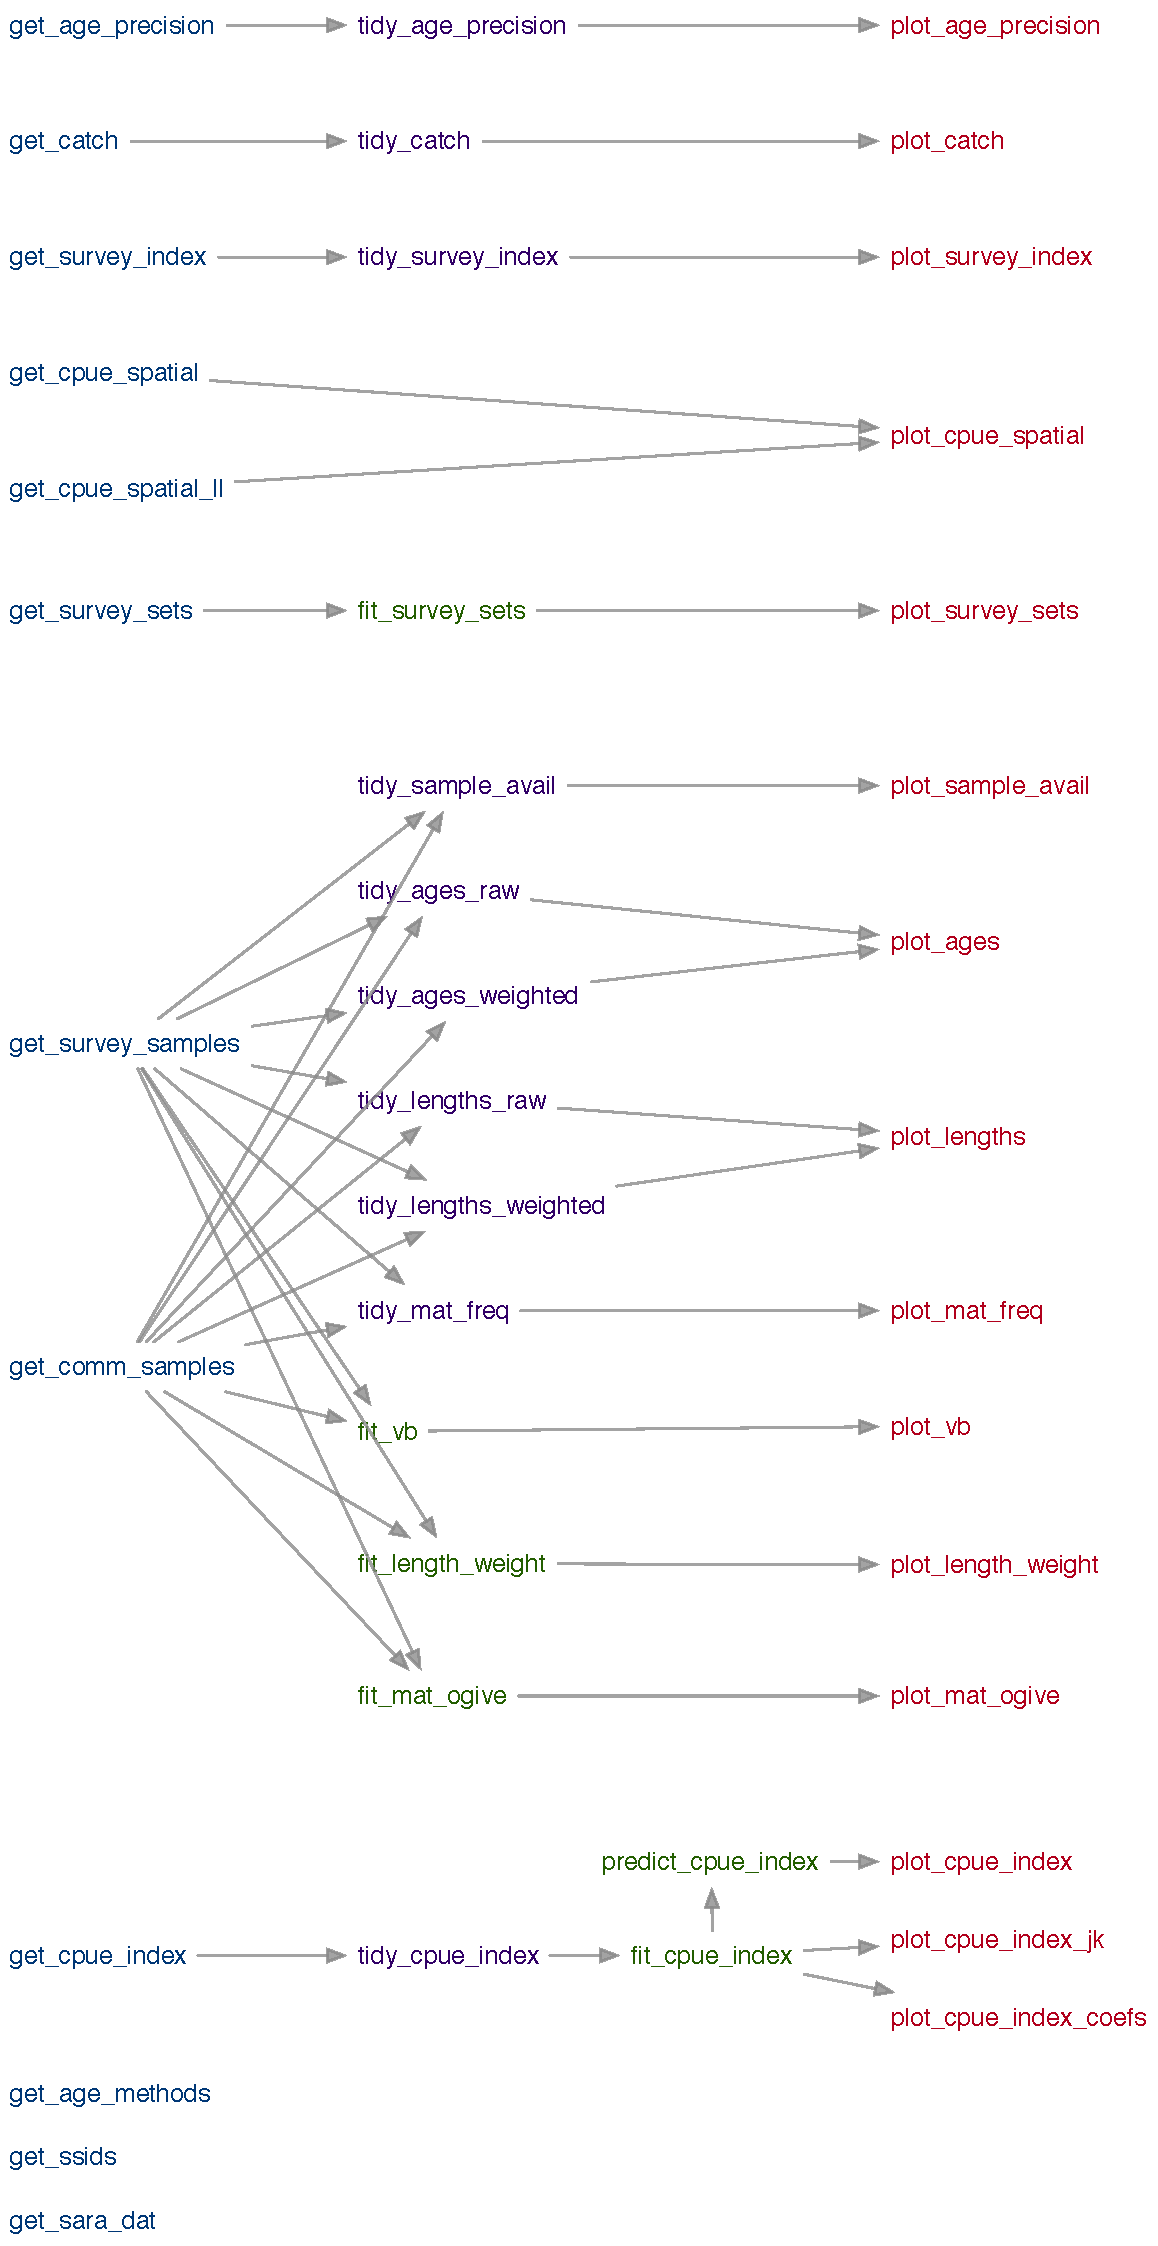
\includegraphics[width=0.65\textwidth]{doc/function-web.pdf}
    \caption{An illustration of the gfplot functions and how they interact.
    \texttt{get} functions extract raw data from the relational databases, \texttt{tidy}
  and \texttt{fit} functions manipulate the data or fit statistical models, and
  \texttt{plot} functions take the output from the tidying or fitting functions to
  make visualizations.}
  \label{fig:gfplot-web}
\end{figure}


\clearpage

\bibliography{spp-refs,synopsis,survey-refs}

\end{document}
